\subsection{Dati e risultati}

\paragraph{Ritardo in commutazione.}

Come tutti i dispositivi elettronici, anche le porte logiche presentano delle non-idealità
che possono creare problemi in alcuni circuiti oppure venir sfruttate in altri. La principale
non idealità delle porte logiche è il ritardo nella commutazione. Più nel dettaglio, essendo le
porte logiche costruite con dei transistor (nella TTL), ogni porta ha una sua piccola capacità
(qualche pF) a causa delle giunzioni PN all'interno dei transistor. La capacità implica che
la risposta della porta non sarà istantanea, ma sarà leggermente in ritardo rispetto al segnale in ingresso,
provocando un ritardo nella commutazione.

Per verificare sperimentalmente questo fenomeno, abbiamo misurato il ritardo nella risposta di una porta NOT.
Il circuito che abbiamo utilizzato è riportato in figura \ref{fig:ritardo10}. Il circuito misura il ritardo generato
da 3 porte NOT (costruite mediante NAND) in sequenza, in modo da aumentare l'entità dell'effetto e tendere più precisa la misura.
La porta NAND in fondo alla serie di NOT trasforma il ritardo in un impulso.

\begin{figure}
        \begin{circuitikz}
                \draw
                    (7, -0.3) node[nand port] (nand) {}
                    (0, 0) node[anchor=east] {IN}
                    to (nand.in 1)
                    (0.5, 0) to (0.5, -1)
                    (2.2, -1) node[nand port] (not1) {}
                    (3.8, -1) node[nand port] (not2) {}
                    (5.4, -1) node[nand port] (not3) {}
                    (0.5, -1) -| (not1.in 1) -| (not1.in 2)
                    (not1.out) -| (not2.in 1) -| (not2.in 2)
                    (not2.out) -| (not3.in 1) -| (not3.in 2)
                    (not3.out) -| (nand.in 2)
                    (nand.out) node[anchor=west] {OUT}
                ;
        \end{circuitikz}
        \caption{Circuito per la misura del ritardo.}
        \label{fig:ritardo10}
\end{figure}

Nello stato iniziale, ovvero ingresso costante 0, la porta NAND ha un uscita uguale a 1, poiché ad
un ingresso riceve direttamente lo 0 e all'altro 1. Quando l'input passa da 0 a 1,
la porta NAND commuta stato e il suo output diventa 0: ad un ingresso c'è 1, mentre all'altro c'è ancora 1 a causa del ritardo delle
porte NOT. Quando anche le porte NOT commutano, la NAND si ritrova con un input 1 e l'altro 0, quindi
l'uscita torna ad essere 1. Al momento della discesa da 1 a 0 non accade nulla.

Idealmente si forma un circuito che da in output un impulso rettangolare di durata pari a quella
della commutazione delle 3 porte. Chiaramente, avendo anche la porta NAND un suo tempo di commutazione
l'impulso in realtà non sarà rettangolare, ma smussato. Per questo è importante usare 3 porte NOT:
in questo modo si evita che il ritardo della porta NAND renda incomprensibile il segnale di uscita,
assicurandoci che la commutazione dei NOT duri circa il triplo di quella della NAND.

Il risultato della misura è mostrato nel grafico in figura \ref{fig:comm_time_10}.
La figura mostra l'input e l'output del circuito \ref{fig:ritardo10}. All'ingresso è stata applicata
un'onda quadra di frequenza 100 kHz tra 0 V e 5 V e la figura mostra il fronte in salita dell'onda.
La commutazione ha una durata di circa 60 ns che significa 20 ns per ciascuna porta NOT.
Questi valori sono in accordo con quelli riportati dal costruttore.

\begin{figure}[t]
    \centering
    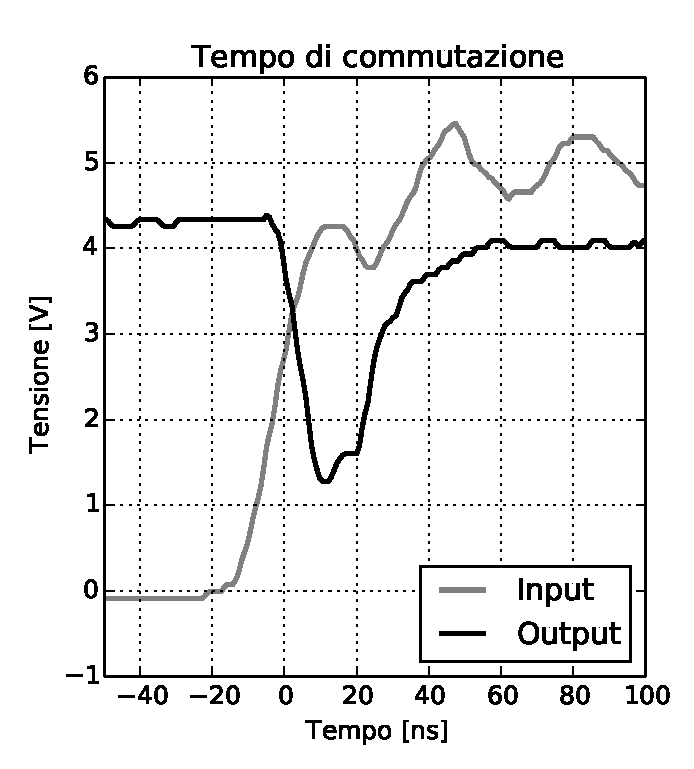
\includegraphics[width=\columnwidth]{figure/comm_time.pdf}
    \caption{}
    \label{fig:comm_time_10}
\end{figure}

\paragraph{Porte open collector.}

Le porte logiche hanno un altra caratteristica che puó creare problemi: possono sostenere
al massimo una certa corrente di output, che spesso è piuttosto limitata e non è quindi adatta
per pilotare carichi che necessitano di grandi correnti, come per esempio un LED.
Possono sorgere problemi anche se una porta logica è utilizzata per pilotare un gran numero di
altre porte logiche. In questo contesto si parla spesso di \emph{fan out} ovvero del massimo
numero di porte della stessa famiglia che una porta è in grado di pilotare.

Per risolvere il problema si ricorre alle porte open collector, ovvero a delle porte
che invece di pilotare l'uscita, pilotano un transistor che ha l'emettitore
collegato a ground mentre il collettore è l'uscita accessibile all'utilizzatore (da qui il nome)
e puó essere collegato all'alimentazione mediante una resistenza dimensionata per
ottenere la corrente desiderata. In questo modo si possono pilotare carichi che richiedono
correnti elevate.

Quello che abbiamo fatto in laboratorio è semplicemente verificare il funzionamento
della porta facendo accendere un LED. Il LED era collegato all'alimentazione (+9 V) e
a una resistenza che era a sua volta collegata alla porta NOT open collector a nostra disposizione.

La resistenza deve essere dimensionata in modo opportuno. La corrente che il LED assorbe è di 5 mA,
inoltre la caduta di potenziale all'interno del LED è di circa 1 V mentre tra collettore
ed emettitore ci sono circa 0.4 V. Imponendo che la corrente debba essere di 5 mA, la resistenza deve essere
circa $(9-1-0.4)/0.005 = 1.52$ \si{\kilo\ohm}. Abbiamo quindi utilizzato una resistenza da 1 \si{\kilo\ohm}
e un trimmer da 1 \si{\kilo\ohm}, in modo da poter regolare la corrente, misurata con il multimetro
mentre la NOT era in funzione, fino al valore desiderato.

In seguito, abbiamo verificato il funzionamento fornendo 0 o 1 in input al NOT e osservando il LED.
Risultato:

\begin{itemize}
    \item{1 in entrata $\implies$ LED acceso.}
    \item{0 in entrata $\implies$ LED spento.}
\end{itemize}

In pratica il transistor è in interdizione se l'entrata è bassa.

\paragraph{Buffer tri-state.}

Un buffer tri-state è un dispositivo che somiglia ad una porta AND (o nel caso del modello 74SL125 una porta NAND).
Un buffer tri-state può essere pensato come un interruttore (come anche una porta AND può essere
considerata un interruttore), e ha 3 connessioni: l'input, l'output e un terminale di controllo.
Nel caso del 74SL125, se il terminale di controllo è a 0, l'input e l'output sono collegati, mentre se è a 1
l'interruttore è aperto. La peculiarità dei buffer tri-state, da cui deriva anche il loro nome, è il fatto
che quando l'interruttore è aperto assumono una configurazione di alta impedenza in uscita, che permette
di creare circuiti che si comportano come se il buffer non esistesse se è aperto.

\begin{figure}
    \centering
    \begin{circuitikz}
                \draw
                        (-0.5, 0.5) node[rground] {}
                        to [sqV] (-0.5, 2)
                        (3, 2) node[buffer] (b1) {} (3, 3) node {B1}
                        (4, 0) node[buffer] (b2) {} (4.5, -0.5) node {B2}
                        (-0.5, 2) to (b1.in)
                        (b1.out) -| (5, 1)
                        (b2.out) -| (5, 1)
                        to [leDo] (7, 1) (6, 1.75) node {LED} (7, 1)
                        to (7, 0) node[rground] {}
                        (b2.in) to (2.75, 0) node[rground] {}
                        (0, -1) node[left] {S}
                        to (1, -1) -| (1, 1) to (3, 1) to (3, 1.4)
                        (3, 1.5) circle (0.1cm)
                        (3, -1.5) node[nand port] (n) {}
                        (1, -1) to (1, -1.5)
                        (1, -1.5) -| (n.in 1)
                        (1, -1.5) -| (n.in 2)
                        (n.out) -| (4, -0.6)
                        (4, -0.5) circle (0.1cm)
                ;
        \end{circuitikz}
        \caption{}
        \label{fig:circ_s10}
\end{figure}

Abbiamo quindi costruito il circuito \ref{fig:circ_s10}. Il circuito serve principalmente per poter sperimentare
il funzionamento dei buffer tri-state. Il circuito è collegato con il generatore di forme d'onda che forniva un onda
quadra 0-5 V di frequenza variabile (per poter vedere l'effetto si deve stare sotto i 10 Hz).
È poi presente una linea di selezione S, che permette di scegliere se aprire il buffer B1 oppure il B2.
Per come il circuito è costruito, se S è a 0 si ottiene che il buffer B1 è aperto, mentre se S è 1 è aperto
il buffer B2.

In pratica il circuito fa passare il segnale, che viene poi visualizzato dal LED se S = 0, mentre il LED è
spento se S = 1. Il circuito ha funzionato a dovere.

\paragraph{Multiplexer}

\begin{figure}
	\centering
	\begin{circuitikz}[transform shape, scale=0.9]
	    \draw
		% Piazzo le NAND
		  (3,0) node[rotate=-90, american nand port] (nand3) {}
		++(1.5,0) node[rotate=-90, american nand port] (nand2) {}
		++(1.5,0) node[rotate=-90, american nand port] (nand1) {}
		++(1.5,0) node[rotate=-90, american nand port] (nand0) {}
	    ;
		% Metto l'output
		\node at (nand3.out) [below] {$Q_3$};
		\node at (nand2.out) [below] {$Q_2$};
		\node at (nand1.out) [below] {$Q_1$};
		\node at (nand0.out) [below] {$Q_0$};
		
		% Coordinate inizio linee
		\coordinate (cS0)  at (0,2) ;
		\coordinate (cS0N) at (0,3)   ;
		\coordinate (cS1)  at (0,4) ;
		\coordinate (cS1N) at (0,5)   ;
		
		% Scrivo gli ingressi
		\node at (cS0)  [left] {$S_0$};
		\node at (cS0N) [left] {$\overline{S_0}$};
		\node at (cS1)  [left] {$S_1$};
		\node at (cS1N) [left] {$\overline{S_1}$};
		    
		% path per intersezioni linee di ingresso
		% Linee:
		\path[name path=S0]  (cS0)  -- ++(12,0);
		\path[name path=S0N] (cS0N) -- ++(12,0);
		\path[name path=S1]  (cS1)  -- ++(12,0);
		\path[name path=S1N] (cS1N) -- ++(12,0);
		% Porte:
		\path[name path=n31] (nand3.in 1) -- ++(0,6);
		\path[name path=n32] (nand3.in 2) -- ++(0,6);
		\path[name path=n21] (nand2.in 1) -- ++(0,6);
		\path[name path=n22] (nand2.in 2) -- ++(0,6);
		\path[name path=n11] (nand1.in 1) -- ++(0,6);
		\path[name path=n12] (nand1.in 2) -- ++(0,6);
		\path[name path=n01] (nand0.in 1) -- ++(0,6);
		\path[name path=n02] (nand0.in 2) -- ++(0,6);
		
		% prima parte (linee e not)
		\draw
		    (cS0N) ++(2,0) node[american not port] (not0) {} 
		    (cS0) ++(1,0) |- (not0.in)
		    (cS1N) ++(2,0) node[american not port] (not1) {} 
		    (cS1) ++(1,0) |- (not1.in)
		;
		
		% definizione di coordinate di partenza per le linee
		\coordinate (nS0)  at (cS0)      ;
		\coordinate (nS0N) at (not0.out) ;
		\coordinate (nS1) at (cS1)       ;
		\coordinate (nS1N) at (not1.out) ;
		
		% S0
		\draw [name intersections={of=n32 and S0, by=x}]
		    (nS0)--(x)--(nand3.in 2);
		\draw [name intersections={of=n22 and S0, by=y}]
		    (x)--(y)--(nand2.in 2);
		    
		% S0N
		\draw [name intersections={of=n12 and S0N, by=x}]
		    (nS0N)--(x)--(nand1.in 2);
		\draw [name intersections={of=n02 and S0N, by=y}]
		    (x)--(y)--(nand0.in 2);            
	    
		% S1
		\draw [name intersections={of=n31 and S1, by=x}]
		    (nS1)--(x)--(nand3.in 1);
		\draw [name intersections={of=n11 and S1, by=y}]
		    (x)--(y)--(nand1.in 1);
		    
		% S1N
		\draw [name intersections={of=n21 and S1N, by=x}]
		    (nS1N)--(x)--(nand2.in 1);
		\draw [name intersections={of=n01 and S1N, by=y}]
		    (x)--(y)--(nand0.in 1);            
		
		
		%(0,1) node[left] {$S_1$} -| (nand1.in 1)
	\end{circuitikz}
	\caption{Circuito di selezione della linea.}
	\label{fig:selezione10}
\end{figure}

Congiuntamente con un altro gruppo, abbiamo realizzato un sistema di Multiplexing/Demultiplexing. Il multiplexing
è una tecnica che consente di trasmettere più segnali attraverso un unico cavo (per esempio per
risparmiare prezioso cavo come nelle linee telefoniche). L'idea di base è questa:
si hanno N diverse segnali digitali da trasmettere. Si inizia trasmettendo il primo segnale e segnalando
all'altro capo, attraverso dei cavi di selezione o di controllo, quale degli N segnali si sta trasmettendo.
Poi si trasmette il secondo segnale, poi il terzo e così via, fino all'N-esimo e poi si ricomincia.
Chiaramente la frequenza del segnale lungo il cavo deve essere N volte quella dei segnali da trasemttere.
Un altro tipo di multiplexing (questo tipo si chiama \emph{time-division multiplexing}) divide le frequenze
invece del tempo.

Noi abbiamo realizzato un multiplexing a 4 linee, cioè in grado di trasmettere fino a 4 segnali diversi.
Abbiamo quindi 4 segnali in entrata, un cavo di collegamento che contiene un filo per la trasmissione, 2 per
la selezione e un filo che trasporta il comune, in modo da non avere trasmittente e ricevente flottanti.
I 2 cavi di selezione sono necessari perché 2 bit codificano 4 diversi stati, corrispondenti a quale delle 4
linee di dati è attiva.

\begin{figure}
	\centering
	\begin{circuitikz}[transform shape, scale=0.78]

	% Nodi inizio linee
		\node (D0) at (0,2) [left] {$D_0$} ;
		\node (D1) at (0,3) [left] {$D_1$} ;
		\node (D2) at (0,4) [left] {$D_2$} ;
		\node (D3) at (0,5) [left] {$D_3$} ;
		
	     % Coordinate fine linee
	     	\coordinate (D0F) at ($(D0)+(9,0)$);
		\coordinate (D1F) at ($(D1)+(9,0)$);
		\coordinate (D2F) at ($(D2)+(9,0)$);
		\coordinate (D3F) at ($(D3)+(9,0)$);
		
	     % Piazzo i buffer
	     	\node (buf0) at ($(D0)+(8,0)$)[buffer] {} ;
	\node (buf1) at ($(D1)+(6,0)$)[buffer] {} ;
		\node (buf2) at ($(D2)+(4,0)$)[buffer] {} ;
		\node (buf3) at ($(D3)+(2,0)$)[buffer] {} ;
		
	     % Tiro le linee
	     	\draw
		(D0) -- (buf0.in) (buf0.out) -- (D0F)
		    (D1) -- (buf1.in) (buf1.out) -- (D1F)
		    (D2) -- (buf2.in) (buf2.out) -- (D2F)
		    (D3) -- (buf3.in) (buf3.out) -- (D3F)
		;
		
	     % Rettangolo
	     	\draw
		($(buf3.in)+(0,-5)$) rectangle ($(buf0.out)+(0,-4.4)$)
		($(buf3)+(0,-5)$) node (Q3) [below] {$Q_3$}
		    ($(buf2)+(0,-4)$) node (Q2) [below] {$Q_2$}
		    ($(buf1)+(0,-3)$) node (Q1) [below] {$Q_1$}
		    ($(buf0)+(0,-2)$) node (Q0) [below] {$Q_0$}
		;
		
	     % Ingressi
	     	\coordinate (S1Q) at ($(buf3.in)+(0,-5.8)$);
		\coordinate (S1I) at ($(D3.east)+(0,-5.8)$);
	    \draw
		(S1Q) -- (S1I) node [left] {$S_1$}
		    ($(S1Q)+(0,-0.8)$) -- ($(S1I)+(0,-0.8)$) node [left] {$S_0$}
		;
		
	     % Metto i pallini
	     	\node (buf3C) at ($(buf3)+(0,-0.55)$) [circle=0.1cm, draw]{};
		\node (buf2C) at ($(buf2)+(0,-0.55)$) [circle=0.1cm, draw]{};
		\node (buf1C) at ($(buf1)+(0,-0.55)$) [circle=0.1cm, draw]{};
		\node (buf0C) at ($(buf0)+(0,-0.55)$) [circle=0.1cm, draw]{};
		
	     % Collego i Q ai pallini
	     	\draw
		(Q3.north) -- (buf3C.south)
		    (Q2.north) -- (buf2C.south)
		    (Q1.north) -- (buf1C.south)
		    (Q0.north) -- (buf0C.south)
		;
		
	     % Linea finale e output
	     	\draw
		(D0F)--(D3F)
		    ($(D0F)!.5!(D3F)$) -- ++(0.5,0) node[right]{$OUT$}
		;
	    
	    % Disegno i pallini di collegamento
	    %	\fill (D3F) circle[radius=0.07cm] ;
	 	%	\fill (D2F) circle[radius=0.07cm] ;
	 	%	\fill (D1F) circle[radius=0.07cm] ;
	 	%	\fill (D0F) circle[radius=0.07cm] ;

	\end{circuitikz}
	\caption{Filtro. Permette solo ad una linea di essere trasmessa.
		Il quadrato in basso indica il selettore.}
	\label{fig:filtro10}
\end{figure}

Il circuito è formato da 2 parti:

\begin{itemize}
    \item{Selettore di linea, mostrato in figura \ref{fig:selezione10}. Questo circuito prende 2 input e
        attiva solo una delle uscite, impostandola a 1. Le uscite non selezionate restano a tensione bassa.}
    \item{Filtro, mostrato in figura \ref{fig:filtro10}. Grazie a 4 buffer tri-state, questo componente lascia
        passare solo uno dei segnali. Ogni buffer deve essere collegato alla corrispondente uscita del selettore,
        in modo da poter selezionare con i terminali di selezione quale dei 4 segnali viene inviato lungo il cavo.}
\end{itemize}

All'altro terminale del cavo è presente un circuito di demultiplexing, che agisce in maniera opposta ed è costruito in
maniera molto simile. Questo componente è stato realizzato dal nostro gruppo partner. Una volta montato il circuito
lo abbiamo testato inviando segnali generati con il generatore di funzioni d'onda, a uno degli input e selezionando
con le linee di selezione i 4 canali a rotazione. L'altro gruppo, mediante una scheda con i LED, ha verificato
la ricezione del segnale. Anche se il circuito è piuttosto intricato, siamo riusciti a realizzarlo
correttamente al primo tentativo.
